\documentclass[conference,twocolumn]{IEEEtran}
\usepackage[utf8]{inputenc}
\usepackage{graphicx}
\usepackage{amsmath}
\usepackage{hyperref}
\usepackage{booktabs}
\usepackage{float}
\usepackage{listings}
\usepackage{xcolor}

\lstset{
  basicstyle=\ttfamily\footnotesize,
  breaklines=true,
  frame=single,
  backgroundcolor=\color{gray!10},
  keywordstyle=\color{blue},
  commentstyle=\color{green!50!black},
  stringstyle=\color{red!70!black},
}

\title{TRS Winter School — Computer Vision Tasks}
\author{Parv Chopra}

\begin{document}
\maketitle

% =====================================================================
\begin{abstract}
This report documents two computer vision tasks completed as part of the TRS Winter School. \textbf{Task~1} implements the RRT* (Rapidly-exploring Random Tree Star) algorithm for path planning on the IIT Kharagpur campus road network, extracting traversable roads from a map image via a multi-stage OpenCV preprocessing pipeline. \textbf{Task~2} uses K-Means clustering to segment an image, identify the background, and replace it with a stock image, similar to a Zoom virtual background. Both tasks demonstrate practical applications of image processing, OpenCV, and algorithmic techniques.
\end{abstract}

% =====================================================================
\section{Introduction}

Computer vision enables machines to extract meaningful information from images. This report covers two tasks that apply different aspects of computer vision:

\begin{enumerate}
    \item \textbf{RRT* Path Planning:} Converting a campus map image into a traversable binary road mask through image processing, then applying the RRT* sampling-based motion planning algorithm to find an optimal path between two points.
    \item \textbf{Background Removal via K-Means:} Using unsupervised clustering to segment image pixels into groups, identifying the background cluster, and replacing it with a stock background.
\end{enumerate}

Both tasks rely heavily on OpenCV for image processing and NumPy for efficient array operations.

% =====================================================================
% TASK 1
% =====================================================================
\section{Task 1: RRT* Path Planning on IIT KGP Campus Map}

\subsection{Problem Statement}

Implement the RRT* algorithm to find an optimal path between two designated points on the IIT Kharagpur campus map. The tree's exploration process must be visualized on the map image. Pre-processing with OpenCV is required to convert the map into a traversable format (identifying roads vs.\ obstacles).

Core topics: Path Planning Algorithms, OpenCV, Motion Planning.

\subsection{Related Work}

RRT* was introduced by Karaman and Frazzoli as an asymptotically optimal extension of the Rapidly-exploring Random Tree (RRT) algorithm~\cite{rrt_medium}. While RRT finds \emph{a} feasible path, RRT* continuously rewires the tree to find shorter paths, converging to the optimal solution as the number of samples approaches infinity.

Standard RRT* operates in open 2D/3D configuration spaces with scattered obstacles. Our setting—navigation on 1px-wide skeleton road masks—required significant adaptations (Section~\ref{sec:task1_approach}).

\subsection{Initial Attempts}

\textbf{Morphological opening for denoising:} After HSV color thresholding, a 3$\times$3 morphological opening was applied to remove noise. This was too aggressive—it eroded thin 1--3\,px road lines, fragmenting the network from $\sim$23 connected components to 231 and destroying connectivity between start and end points.

\textbf{Lesson:} Standard morphological operations are unsuitable for structures thinner than the kernel. Gaussian blur + re-thresholding was adopted instead, as it averages pixel values without structural erosion.

\subsection{Final Approach}
\label{sec:task1_approach}

The solution consists of two stages: (1)~a multi-stage preprocessing pipeline that converts the campus map into a clean binary road mask, and (2)~a skeleton-aware RRT* planner.

\subsubsection{Preprocessing Pipeline}

The pipeline converts a campus map image into a 1px-wide skeleton road mask through five stages:

\begin{enumerate}
    \item \textbf{HSV Color Thresholding:} Road lines are blue-ish, which is isolated using HSV bounds $H \in [80, 150]$, $S \geq 10$, $V \geq 50$. HSV separates color from brightness, making it robust to lighting variations.
    
    \item \textbf{Small Component Removal:} \texttt{cv2.connectedComponentsWithStats} with 8-connectivity removes components with area $< 18$\,px (noise dots) while preserving contiguous road structures.
    
    \item \textbf{Gaussian Blur Denoising:} A 3$\times$3 Gaussian blur followed by re-thresholding at 127. Isolated white pixels surrounded by black are averaged below the threshold and disappear, while connected road lines survive.
    
    \item \textbf{HoughLinesP Gap Filling:} \texttt{cv2.HoughLinesP} detects line segments and bridges gaps up to 5\,px between disconnected road fragments. This runs \emph{before} skeletonization because Hough requires multi-pixel-wide lines for reliable detection.
    
    \item \textbf{Skeletonization:} Zhang-Suen morphological thinning (\texttt{skimage.morphology.skeletonize}) reduces all roads to 1px-wide center lines, producing a clean topology with no redundant parallel paths.
\end{enumerate}

The pipeline order is critical: each stage depends on the previous one's output characteristics.

\begin{table}[ht]
\centering
\caption{Preprocessing Parameters}
\label{tab:preprocess_params}
\begin{tabular}{@{}lll@{}}
\toprule
\textbf{Parameter} & \textbf{Value} & \textbf{Purpose} \\
\midrule
HSV range & (80,10,50)–(150,255,255) & Road color detection \\
Min component area & 18\,px & Remove noise dots \\
Hough threshold & 12 & Min votes for a line \\
Min line length & 10\,px & Filter short fragments \\
Max line gap & 5\,px & Bridge disconnected roads \\
\bottomrule
\end{tabular}
\end{table}

\subsubsection{RRT* Algorithm}

The RRT* planner builds a space-filling tree from a start point toward a goal, continuously optimizing path cost through rewiring.

\textbf{Per-iteration loop:}
\begin{enumerate}
    \item \textbf{Sample} a random road pixel (or the goal with probability $p_{\text{goal}} = 0.05$).
    \item \textbf{Find nearest} tree node via KDTree — $O(\log n)$.
    \item \textbf{Steer} from nearest toward sample by \texttt{step\_size} pixels, then \textbf{snap} to the nearest road pixel.
    \item \textbf{Collision check} the edge on the dilated mask.
    \item \textbf{Choose best parent} among nearby nodes within \texttt{rewire\_radius} that minimizes cost.
    \item \textbf{Rewire} — reroute nearby nodes through the new node if it reduces their cost.
    \item If within \texttt{goal\_radius} of the goal, record the path.
\end{enumerate}

\subsubsection{Skeleton-Aware Adaptations}

Two key adaptations were required for 1px skeleton masks:

\textbf{1. Snap-to-Road Steering:} When RRT* steers toward a sampled point, the result almost never lands on a 1px line. The steered point is snapped to the nearest road pixel via a KDTree built over all road pixel coordinates:
\begin{equation}
    p_{\text{new}} = \arg\min_{r \in \text{road}} \| p_{\text{steered}} - r \|_2
\end{equation}

\textbf{2. Dilated Collision Mask:} Two nodes on a curving skeleton may have a straight-line connection that briefly passes through a non-road pixel. A 2-iteration dilation creates $\sim$5px corridors for collision checking:
\begin{equation}
    M_{\text{collision}} = \text{dilate}(M_{\text{skeleton}}, K_{3\times3}, \text{iter}=2)
\end{equation}

\subsubsection{KDTree Data Structure}

A \textbf{KDTree} (K-Dimensional Tree) is a binary space-partitioning data structure used to organize points in $k$-dimensional space. At each level of the tree, the points are split along one axis (cycling through dimensions), creating a balanced binary tree. This enables nearest-neighbor queries in $O(\log n)$ average time instead of $O(n)$ brute-force search.

In our implementation, two KDTrees are used:
\begin{itemize}
    \item \textbf{Tree-node KDTree:} Built over all RRT* tree nodes. Used to find the nearest existing node to a newly sampled point. Rebuilt periodically as the tree grows.
    \item \textbf{Road-pixel KDTree:} Built once over all road pixel coordinates. Used for snap-to-road steering — finding the nearest road pixel to a steered point in $O(\log m)$ time ($m$ = number of road pixels).
\end{itemize}

\subsubsection{Optimizations}

\begin{itemize}
    \item \textbf{Informed sampling:} Only samples from road pixels, never from obstacle space.
    \item \textbf{KDTree acceleration:} $O(\log n)$ nearest-neighbor via \texttt{scipy.spatial.KDTree}, rebuilt periodically.
    \item \textbf{Auto-computed parameters:} Step size, goal radius, rewire radius, and max iterations are all computed from \texttt{dim = max(width, height)}, enabling the same script to work on any map size.
    \item \textbf{Goal bias:} 5\% of samples target the goal directly.
\end{itemize}

\begin{table}[ht]
\centering
\caption{RRT* Auto-Computed Parameters}
\label{tab:rrt_params}
\begin{tabular}{@{}lll@{}}
\toprule
\textbf{Parameter} & \textbf{Formula} & \textbf{416px} \\
\midrule
Step size & $\max(3, \lfloor \text{dim} \times 0.005 \rceil)$ & 3 \\
Goal radius & $\max(8, \lfloor \text{dim} \times 0.02 \rceil)$ & 8 \\
Rewire radius & $\max(15, \lfloor \text{dim} \times 0.025 \rceil)$ & 15 \\
Max iterations & $\max(50000, \text{dim} \times 100)$ & 50,000 \\
Goal bias & 0.05 (constant) & 0.05 \\
\bottomrule
\end{tabular}
\end{table}

\subsection{Results and Observations}

The processing demo successfully finds a path between the designated start point $(15, 100)$ and end point $(380, 188)$ on the cropped campus map.

\begin{table}[ht]
\centering
\caption{Task 1 Results}
\label{tab:task1_results}
\begin{tabular}{@{}ll@{}}
\toprule
\textbf{Metric} & \textbf{Value} \\
\midrule
Road mask coverage & $\sim$7.5\% of image \\
Goal reached & Yes (iteration $\sim$12,475) \\
Final path cost & $\sim$437.2\,px \\
Tree nodes at completion & $\sim$50,000 \\
\bottomrule
\end{tabular}
\end{table}

An additional OSM-based demo validates the same RRT* planner on a larger 800$\times$800 map downloaded from OpenStreetMap, reaching the goal at iteration $\sim$35,221 with a path cost of $\sim$1236\,px.

\begin{figure}[ht]
\centering
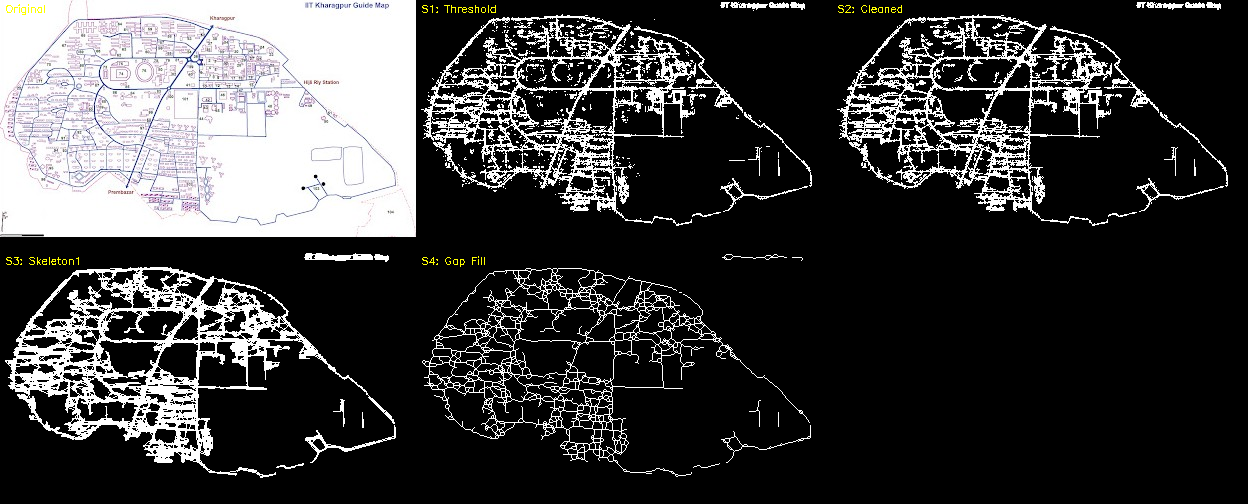
\includegraphics[width=\columnwidth]{task1/processing_demo/output/pipeline_comparison.png}
\caption{Preprocessing pipeline stages: (left to right) HSV threshold, cleaned, denoised, gap filled, skeleton, final road mask.}
\label{fig:pipeline}
\end{figure}

\begin{figure}[ht]
\centering
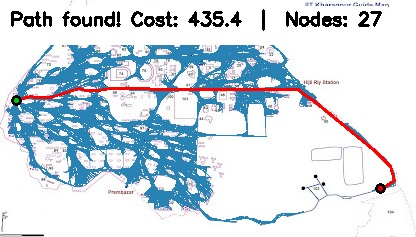
\includegraphics[width=\columnwidth]{task1/processing_demo/output/rrt_star_result.jpg}
\caption{RRT* result on the campus map. The red line shows the optimal path found between start and end points. The blue tree shows the explored nodes.}
\label{fig:rrt_result}
\end{figure}

\subsection{Future Work}

\begin{itemize}
    \item \textbf{Bidirectional RRT*:} Growing trees from both start and goal simultaneously could dramatically reduce convergence time.
    \item \textbf{Weighted sampling:} Biasing samples toward under-explored regions of the road network.
    \item \textbf{Better image preprocessing:} Using adaptive thresholding or learned color models to improve road detection accuracy across varying map styles.
    \item \textbf{Custom line detection:} Developing a domain-specific line detection algorithm tailored to campus map road characteristics, rather than relying on generic HoughLinesP.
\end{itemize}

% =====================================================================
% TASK 2
% =====================================================================
\section{Task 2: Background Removal via K-Means Clustering}

\subsection{Problem Statement}

Use K-Means clustering to segment an image, identify the background cluster, and remove it. Replace the removed background with a stock image (similar to a Zoom virtual background). Images with a significant, roughly uniform background should be chosen to ensure the background is identified as one of the largest clusters.

Core topics: Image Processing, OpenCV, Unsupervised Learning.

\subsection{Related Work}

K-Means clustering is a widely used unsupervised learning algorithm that partitions data into $K$ groups by minimizing within-cluster variance. When applied to image pixels represented as color vectors, it effectively segments images by color similarity. Alternative approaches include semantic segmentation with deep learning and chroma keying (green screen removal).

K-Means offers a simple, interpretable baseline that requires no training data and works well when the background is roughly uniform in color.

\subsection{Initial Attempts}

Initial experiments used CIE LAB color space for clustering. LAB is perceptually uniform—equal Euclidean distances correspond to equal perceived color differences—making it a natural choice. However, for images where foreground and background share similar lightness values, HSV proved more effective at separating clusters by isolating the hue channel.

The initial version identified only the single largest border cluster as background. For images where the background spans multiple shades, this left residual background regions. Extending to the \textbf{two most border-dominant clusters} resolved this issue.

\subsection{Final Approach}

\subsubsection{K-Means Clustering in Color Space}

The image is Gaussian-blurred (5$\times$5 kernel) to reduce noise, then converted to a perceptually meaningful color space. Each pixel becomes a 3D feature vector, and OpenCV's \texttt{cv2.kmeans} partitions all pixels into $K$ clusters using K-Means++ initialization, run 10 times to avoid poor local minima.

The K-Means objective minimizes:
\begin{equation}
    J = \sum_{i=1}^{K} \sum_{x \in C_i} \| x - \mu_i \|^2
\end{equation}
where $C_i$ is cluster $i$ and $\mu_i$ is its centroid.

\subsubsection{Background Cluster Identification}

A \textbf{border-dominance heuristic} identifies the background: pixels along all four image edges are collected, and the two cluster labels most frequent on the border are selected as background clusters. This works because background regions typically extend to the image edges.

\subsubsection{Foreground Mask Generation}

A binary mask is created where all pixels belonging to the two background clusters are set to 0 (background) and all others to 255 (foreground). The mask is then cleaned:

\begin{enumerate}
    \item \textbf{Morphological closing} (elliptical 7$\times$7 kernel, 3 iterations): Fills small holes inside the foreground.
    \item \textbf{Morphological opening} (same kernel, 3 iterations): Removes small noise blobs.
    \item \textbf{Gaussian feathering} ($\sigma = 5$\,px): A Gaussian blur is applied to the binary mask edges. This converts the hard 0/255 boundary into a smooth gradient, producing partial transparency at the foreground-background transition. Without feathering, composited edges appear jagged and unnatural; with it, the foreground blends seamlessly into the replacement background.
\end{enumerate}

\subsubsection{Compositing}

The replacement background is resized to match the input dimensions. The final result is an alpha blend:
\begin{equation}
    I_{\text{result}} = \alpha \cdot I_{\text{fg}} + (1 - \alpha) \cdot I_{\text{bg}}
\end{equation}
where $\alpha$ is the feathered mask normalized to $[0, 1]$.

\begin{table}[ht]
\centering
\caption{Task 2 Configuration Parameters}
\label{tab:task2_params}
\begin{tabular}{@{}lll@{}}
\toprule
\textbf{Parameter} & \textbf{Value} & \textbf{Purpose} \\
\midrule
$K$ & 3 & Number of clusters \\
Blur kernel & 5$\times$5 & Pre-clustering noise reduction \\
Morph kernel & 7$\times$7 & Mask cleanup \\
Morph iterations & 3 & Close/open iterations \\
Feather $\sigma$ & 5\,px & Edge softening \\
\bottomrule
\end{tabular}
\end{table}

\subsection{Results and Observations}

The pipeline successfully segments the input image, identifies the background via border dominance, and produces a clean composite with the replacement abstract background. The Gaussian-feathered mask creates smooth, natural transitions at foreground-background boundaries, avoiding the harsh cut-out look that a binary mask would produce.

\begin{figure}[ht]
\centering
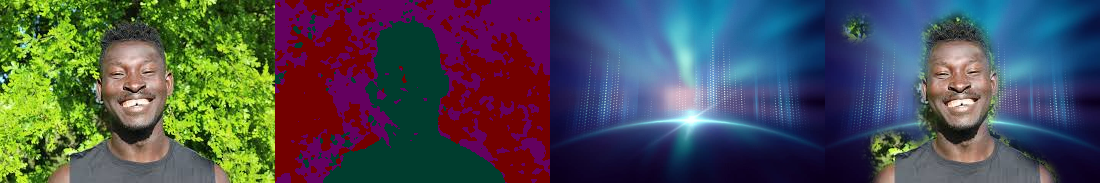
\includegraphics[width=\columnwidth]{task2/output/comparison.png}
\caption{Task 2 pipeline: (left to right) original image, K-Means segmented clusters, replacement background, final composite result.}
\label{fig:kmeans_result}
\end{figure}

\begin{figure}[ht]
\centering

\includegraphics[width=0.6\columnwidth]{task2/output/foreground_mask.png}
\caption{Foreground mask generated by K-Means background identification and morphological cleanup.}
\label{fig:fg_mask}
\end{figure}

Removing the \textbf{two} most border-dominant clusters (rather than one) handles cases where the background spans multiple color shades, such as gradient backgrounds or shadows near edges.

\textbf{Trade-offs:}
\begin{itemize}
    \item Increasing $K$ can separate finer foreground details but may fragment the background into multiple clusters.
    \item $K = 3$ is default as it provides good separation for images with a dominant background.
    \item The border heuristic fails when the foreground subject touches the image border—manual cluster selection or spatial features would be needed in such cases.
\end{itemize}

\subsection{Future Work}

\begin{itemize}
    \item \textbf{Spatial features:} Including $(x, y)$ coordinates in the feature vector to make clustering spatially aware.
    \item \textbf{Adaptive $K$:} Using the elbow method or silhouette score to automatically determine $K$.
    \item \textbf{Boundary-aware detection:} Handling cases where the foreground subject touches or overlaps with image boundaries, where the border-dominance heuristic may misclassify foreground pixels as background.
    \item \textbf{Real-time processing:} Optimizing for video streams (frame-to-frame coherence).
\end{itemize}

% =====================================================================
\section{Conclusion}

This report presented two computer vision tasks. Task~1 demonstrated a complete pipeline from raw map image to optimal path planning, combining multi-stage image preprocessing with a skeleton-aware RRT* algorithm. Key innovations included Gaussian blur denoising for thin structures and snap-to-road steering for skeleton masks. Task~2 showed how unsupervised K-Means clustering can be used for background segmentation and replacement, with border-dominance heuristics and morphological cleanup producing clean results comparable to commercial virtual background tools. Both tasks highlight the versatility of OpenCV and fundamental computer vision techniques in solving real-world problems.

% =====================================================================
\begin{thebibliography}{9}

\bibitem{rrt_medium}
T.~Erickson, ``Robotic Path Planning: RRT and RRT*,'' Medium, 2019. [Online]. Available: \url{https://theclassytim.medium.com/robotic-path-planning-rrt-and-rrt-212319121378}

\end{thebibliography}

\end{document}
